\section{Experimental Evaluation}
In this section we experimentally evaluate  Crypt$\epsilon$ to assess its practical utility  based on two parameters, the accuracy and the performance of the Crypt$\epsilon$ programs. Specifically the experiments were designed to answer the following questions:
\begin{enumerate}\item Does Crypt$\epsilon$ programs have constant error bounds depending only on the privacy parameter $\epsilon$  which is at least $O(\sqrt{m})$ times lower than that for the corresponding state-of-the-art LDP implementation? \item Is the program execution timings for Crypt$\epsilon$ practical? \item Does the proposed DP- optimizations provide substantial performance improvement over the base case Crypt$\epsilon$ implementation? \end{enumerate}

\paragraph{Methodology:} To answer the aforementioned questions we ran the experiments on the 7 Crypt$\epsilon$ programs previously outlined in section 5. We ran our experiments on a dataset which is generated from the UCI Adult dataset by randomly sampling 1000 records. The experiment numbers are reported as the mean value after 10 repetitions.
\subsection{Accuracy}
\begin{figure*}
    \centering
    \begin{subfigure}[b]{0.2\textwidth}
        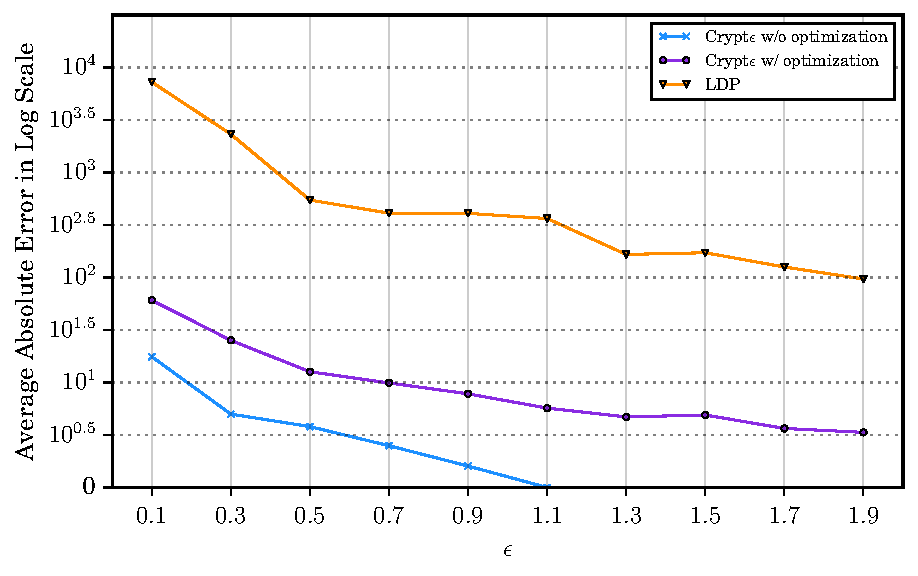
\includegraphics[width=5cm,height=5cm]{test1_1.pdf}
        \caption{ Program 1}
        \label{fig:gull}
    \end{subfigure}\quad \qquad\quad \\%
    ~ %add desired spacing between images, e. g. ~, \quad, \qquad etc.
      %(or a blank line to force the subfigure onto a new line)
    \begin{subfigure}[b]{0.3\textwidth}
       \qquad 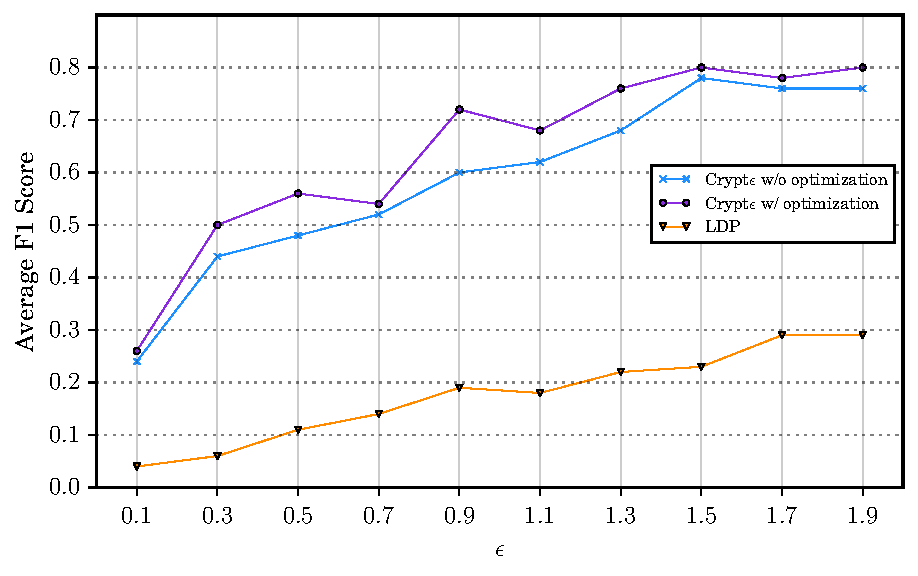
\includegraphics[width=5cm,height=5cm]{test2.pdf}
        \caption{ Program 2}
        \label{fig:tiger}
    \end{subfigure}
    ~ %add desired spacing between images, e. g. ~, \quad, \qquad etc.
      %(or a blank line to force the subfigure onto a new line)
    \begin{subfigure}[b]{0.3\textwidth}
    \qquad    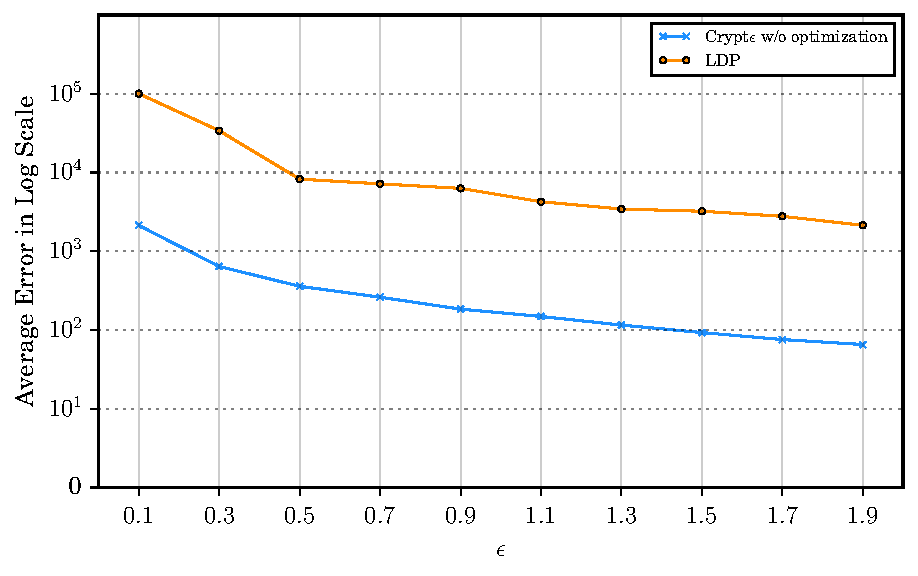
\includegraphics[width=5cm,height=5cm]{test3.pdf}
        \caption{Program 3}
        \label{fig:mouse}\end{subfigure}
          \begin{subfigure}[b]{0.3\textwidth}
    \qquad    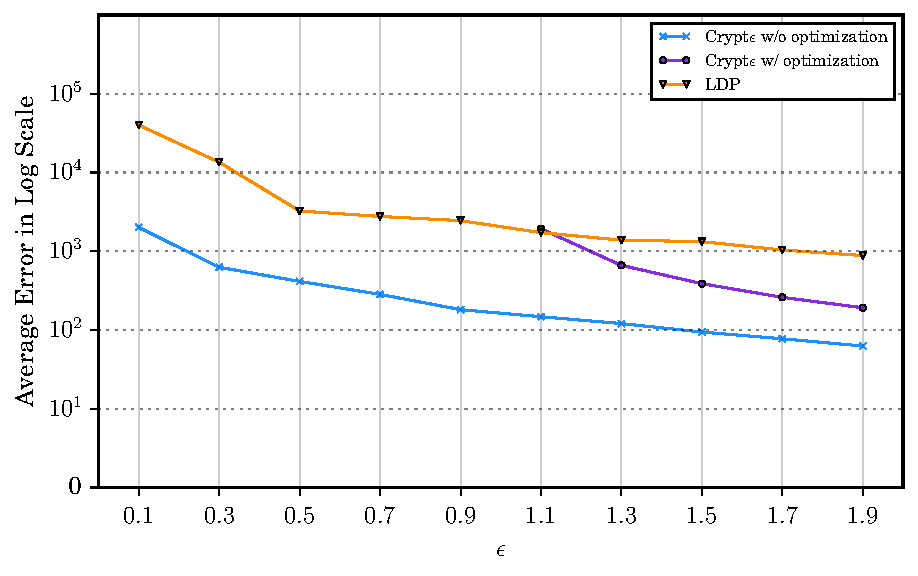
\includegraphics[width=5cm,height=5cm]{test4.pdf}
        \caption{Program 4}
        \label{fig:mouse}\end{subfigure}
          \begin{subfigure}[b]{0.3\textwidth}
    \qquad    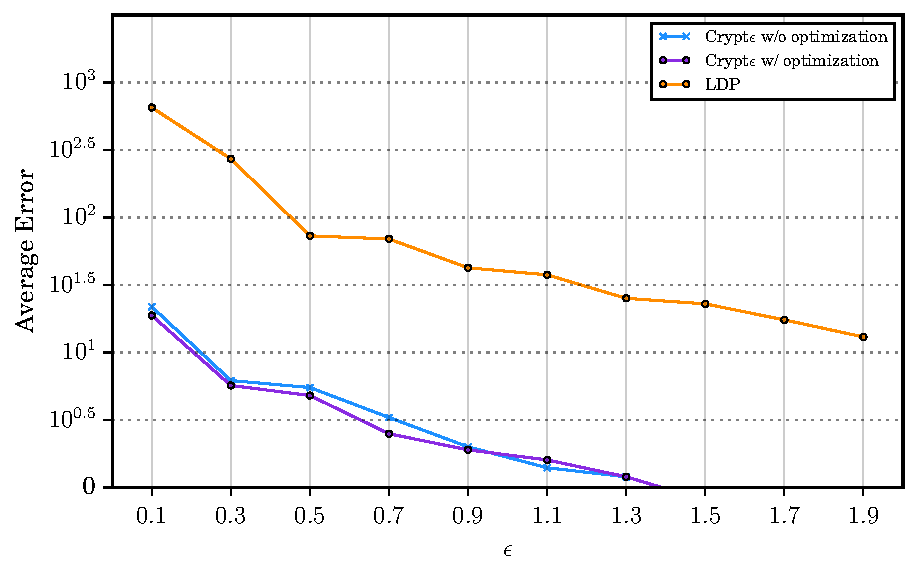
\includegraphics[width=5cm,height=5cm]{test5.pdf}
        \caption{Program 5}
        \label{fig:mouse}\end{subfigure}
          \begin{subfigure}[b]{0.3\textwidth}
    \qquad    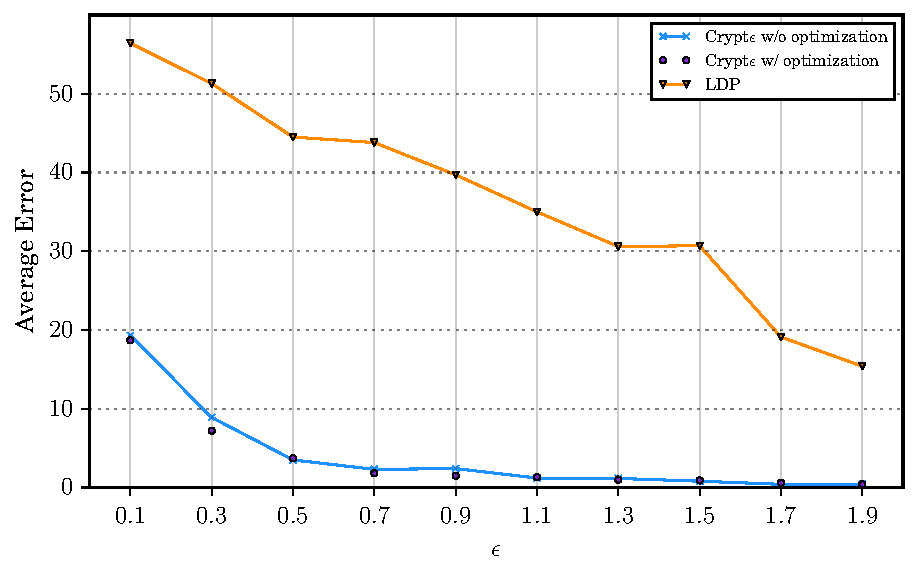
\includegraphics[width=5cm,height=5cm]{test6.pdf}
        \caption{Program 6}
        \label{fig:mouse}\end{subfigure}
          \begin{subfigure}[b]{0.3\textwidth}
    \qquad    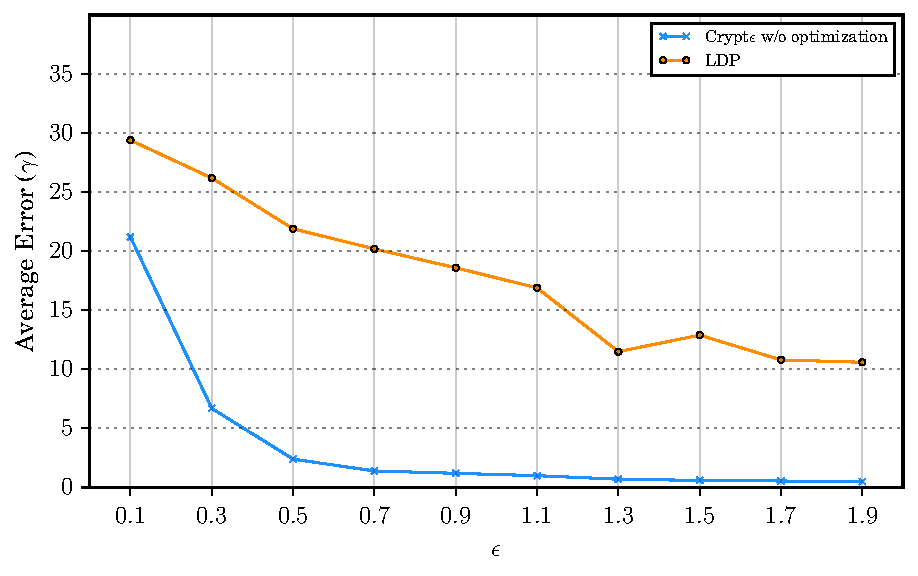
\includegraphics[width=5cm,height=5cm]{test7.pdf}
        \caption{Program 7}
        \label{fig:mouse}
    \end{subfigure}
%    \caption{a) External alignment is the neighborhood of read $X$ in the full genome and $\lambda$ is the \% of $X$ that correctly identifies it. (b) Internal alignment is the index-to-index alignment within the neighborhood of $X$ and $\sigma=avg_i\frac{TBScore_{opt}-TBScore_i}{TBScore_{opt}}$ where $TBScore_{i}=\sum_{[i,j] \in \textit{Traceback path}}\mathbf{M}[i,j]$. 
%   (c) $\rho$ is the number of reads required to cover a single index such that Pr( SNPs are aligned correctly in $Y) > 0.95$}
   \caption{Accuracy Analysis}
\end{figure*}
\textit{Crypt$\epsilon$ Program 1}\\
Program 1 counts the number of records having age in range [50,60].  
\\\textit{LDP } - The competing LDP implementation uses the frequency oracle of \cite{LDP1}. 
\\\textit{Error Measure} - Standard deviation of 
\\\textit{}
\\\textit{Observations} - From Figure 1 we can see that the base case Crypt$\epsilon$ .  
\\\textit{Crypt$\epsilon$ Program 2} - The \\
\textit{Crypt$\epsilon$ Program 3}\\
\textit{Crypt$\epsilon$ Program 4}\\
\textit{Crypt$\epsilon$ Program 5}\\
\textit{Crypt$\epsilon$ Program 6}\\
\textit{Crypt$\epsilon$ Program 7}\\

\subsection{Performance}
In we report the timing . 
Thus we see that are feasible
\begin{table}[ht]
\caption{Computation Time Analysis for Crypt$\epsilon$ Programs}
\centering
\begin{tabular}{c c c c c c c}
\hline\hline
Program &  \multicolumn{3}{c}{Unoptimized} & \multicolumn{3}{c}{Optimized} \\ 
 & AS &  CSP & Total & AS & CSP & Total \\ &(s)&(s)&(s)&(s)&(s)&(s)\\ % inserts table %heading
\hline
1 & 0.49& 0.0027& 0.4927 & 0.0002 &0.0027 & 0.0029 \\
2 &  6.12 & 0.3  &6.42 &0.57&0.32& 0.89\\ %197 the communication rounds
3&  6482.67 & 17435.8 & 23918.47&N/A&N/A &N/A \\4  &8227.89&3761.98&11,989.87&190.57&88.75& 279.32\\5&2.78&2.7&5.48&18.86&17.52&36.38\\6&1910.01&571.11&2481.12&333.91&96.01&429.92\\7&6.35 & 1393.89 & 1400.24 &  N/A & N/A & N/A\\ [1ex]
\hline
\end{tabular}
\label{c}
\end{table}




